\documentclass{report}
\usepackage{graphicx}
\usepackage{adjustbox}
\usepackage{makecell}
\usepackage{hyperref}
\usepackage{boldline}
\usepackage{array}
\usepackage{longtable}
\usepackage{wrapfig}
\usepackage{rotating}
\usepackage{bookmark}

\begin{document}

\title{Project Three Specification}
\author{Connor Byrd, Chad Baxter, Chris Vasquez}
\date{\today}
\maketitle

\tableofcontents

\renewcommand\thesection{\arabic{section}}
\renewcommand\thesubsection{\thesection.\arabic{subsection}}
\renewcommand\thesubsubsection{\thesubsection.\arabic{subsubsection}}

\clearpage

\section{Introduction}

This specification describes the implementation of a multi-user part warehouse application. In this document you can find diagrams and information regarding the creation of this application as well as how this application handles the tasks it is given. \par

\subsection{Document Purpose}

The purpose of this document is to relay to the customers of this program what its capabilities are, and relay to the users of the program how they may use those capabilities. The program's scope, functions, design, and an overall description will be given in distinct sections throughout this document.\par

\subsection{System Scope}

This system is designed to be used by the owners and employees at a bike part distributorship, where bike parts and biking attire are sold to customers for comfort and performance. This system will be able to manage which employee sells which item and total the total sales by each worker. The manager of that shop/distributorship will then be able to generate an invoice for each employee to efficiently calculate the total pay that employee has earned, including commissions. In order to manage which employee is selling a part, each employee will create their own unique login account with a username and password, where no duplicate usernames will be allowed. System admins will create a more thoroughly defined account, using first and last name, an email address, a user name and a password. Once logged in, the employee will enter the part they sold via part name or part number, and the system will calculate for how much that part is sold for and attach that sale to that employee for invoice generation later. Once the employee logs out, the system will remain running for the next employee to log in and make another sale.\par
Once logged in, an employee will be able to add or remove parts from the warehouse inventory and place it in their sales van to move the part and deliver it to a customer. This move will be possible from a main warehouse to a store warehouse, from store warehouse to sales van, and from sales van to sales van. After that, moving from sales van to customer will be considered a sale. The employee will be able to look up a particular part via part name or part number, and this search will display all of that parts attributes (part name, part number, list price, sales price, whether it is on sale or not, and the quantity available). This will allow them to more easily find a part for a sale, and check if the part is available to sell from a particular warehouse/sales van. If an employee wants to view an organized list of everything available to sell to a customer, that is also possible.\par

\subsection{Overview}

Each section in this document is divided into numbered and labeled sections in order to ease the search for the desired information. Each section down the document gets more specific about the program and its capabilities. For questions about system functionality, see Product Functions. For questions about operational design, see System Specification. For questions about the environment this system is meant to run in, see Assumptions.\par

\section{Overall Description}

\subsection{Client Characteristics}

A distributorship needs a way of tracking and maintaining inventory and sales information. This application attempts to provide all functionality needed to properly maintain the client's past, current, and future inventory and sales.\par

\subsection{User Characteristics}

The intended users of this application are distributorship type businesses with small to medium inventories. The application will be used to makes sales of parts and items to other companies and individuals. It is assumed that users have a basic knowledge of how payment transactions work as this application will not handle actual payments or methods of payments.\par

\subsection{Product Functions}

This software is not only designed to manage sales and monetary summations, but also distinguishes between who is doing what with the program. This section will be divided into five main sections; one for system admins (SA), one for an office manager (OM), the warehouse manager (WM) and one for employees. The fifth section will be a list of every command the program can execute and a description of what each command does.\par

\subsubsection{System Admin}

There can be multiple SA’s. Ideally these are the managers of a particular store/warehouse. The primary rolls of an SA are to manage invoices, employee accounts and an office manager account.\par
\begin{description}
  \item [\textit{Invoices}] The system admin will designate a window of time (i.e. every two weeks) in which sales from each sales associate/employee are counted and saved (including the appropriate commission). After that window close, the system admin will create an invoice for each employee which contains the employee name, each sale that employee made (part names listed) and the money collected from each part sold. The invoice will display all of this information and a summation of the money to be paid to that employee for that window of time (pay period).
  \item [\textit{Employee Accounts}] The system admin will create and delete new employee and OM accounts, and will also be in charge of changing passwords, email addresses and/or first and last names for an existing account. Usernames cannot be changed for an existing account.\par
  \item [\textit{Office Manager Account}] There can be only one office manager account per office. The SA will create this account with the individual designated to this account, and delete this account if that individual becomes no longer attached to the company or is moved to another position within the company.\par
\end{description}

\subsubsection{Office Manager}

The office manager will manage warehouse inventory stocks and commission rates.\par
\begin{description}
  \item [\textit{Inventory Stocks}] The OM will be able to search for parts within his/her warehouse via part name or part number. This will display all of that parts attributes including quantity. When the stock of a part is getting low, the office manager will be able to order more of that part to maintain that parts inclusion in the inventory. This can be done for multiple parts at a time if there is more than one part that has fallen below or is near the minimum quantity (set by the OM).\par
  \item [\textit{Commission}] the system admin will determine whether commission will be a part of a sale, what the commission rate is, and which merchandise are included in this commission sale.\par
\end{description}

\subsubsection{Warehouse Manager}

The warehouse manager will be able to view the entire contents of their warehouse and update the inventory of that warehouse.\par
\begin{description}
  \item [\textit{View Inventory}] The WM will be able to view the inventory by inputting a search filter, be it the part name, part number or a quantity. Searching by quantity will allow the WM to view any part that is greater than/less than/equal to the value they input.\par
  \item [\textit{Update Inventory}] Allows the WM to update the electronic inventory list after a delivery has been made to the warehouse.\par
\end{description}

\subsubsection{Employee}

Employees will load sales vans and add their sales to an invoice.\par
\begin{description}
  \item [\textit{Load Van}] The employee will remove parts from a warehouse and put those parts in a sales van to be delivered to the customer.\par
  \item [\textit{Sales Invoice}] An employee will create a list of each part sold, the price it was sold for, who it was sold to, and the total worth of the sale. This will be used by the SA at the end of the pay period to determine pay for each employee.\par
\end{description}

\subsubsection{Commands}

\begin{description}
  \item [\textit{Log In}] Process the username and password, determine what type of account those strings are linked to and open the correct tab for that user.
  \item [\textit{Generate Invoice}] Collects every sale made within the pay period and the accounts linked to the employee that made the sale. Generates one single coagulated invoice for each employee that displays the contents of each sale invoice for that employee, and sums the total pay that employee earned for that pay period.
  \item [\textit{Add Employee}] Create a new account that will be linked to an employee level account, which only has permission to execute the commands given within the section for employees.
  \item [\textit{Add Office Manager}] Create a new account that will be linked to an employee level account, which only has permission to execute the commands given within the section for Office Manager.
  \item [\textit{Add Warehouse Manager}] Create a new account that will be linked to an employee level account, which only has permission to execute the commands given within the section for Warehouse Manager.
  \item [\textit{Add Warehouse}] Generates a new point at which parts can be stored and removed from for sales. WM’s, OM’s and employees will have access to these parts.
  \item [\textit{Add Sales Van}] Generates a new sales van that can be used for sales by employees.
  \item [\textit{Move Part}] Used by employees to load a sales van for a sale. This removes the appropriate quantity of each specified part from the warehouse and adds it to the inventory of the sales van to be sold.
  \item [\textit{Display Part}] Can be used by WM, OM, and employees. Allows the user to display.
  \item [\textit{Sort Parts (Name)}] Sorts the parts in the desired location in alphabetical order.
  \item [\textit{Sort Parts (Number)}] Sorts the parts in the desired location by the part numbers.
  \item [\textit{Sell Parts}] Used by employees. Removes a part from a sales van and adds that part to the invoice for that sale (part name, part number, price sold for).
  \item [\textit{Order Parts}] Used by the OM. Adds a specified part to the warehouse they manage.
  \item [\textit{Update Inventory}] Used by WM. Reads a file containing the origin and destination for a list of parts (this list can be one part long, or many parts long), removes those parts (by the correct quantity) and adds them to the destination warehouse .
  \item [\textit{Set Commission}] Used by OM. Will create a reference to individual parts that, when sold, will increase the pay for the employee that makes the sale, but does not increase the cost of the part. Will be set as a percentage.
\end{description}

\begin{table}[htb]
  \begin{center}
      \begin{tabular}{ | l | p{8cm} |}
      \hline
      User Type & Available Commands \\ \hline
      System Admin & Log In, Generate Invoices, Add Employee, Add Office Manager, Add Warehouse Manager, Add Warehouse, Add Sales Van \\ \hline
      Office Manager & Log In, Set Commission\\ \hline
      Warehouse Manager & Log In, Order Parts, Update Inventory \\ \hline
      Employee & Log In, Move Part, Display Part, Sort Part (Name, Number), Sell Part \\
      \hline
      \end{tabular}
  \end{center}
  \caption{Permission table.}
\end{table}

\section{System Specification}

\begin{enumerate}
  \item \textbf{Factories} Each factory class is a singleton, allowing only one instance at a given time. This ensures that no data is overwritten from a previous command, and instead a new one is made and then stored separately.
    \begin{description}
      \item [InvoiceFactory] Stores and creates all invoices.
      \item [BundleFactory] Stores and creates bundles created when items are made a part of commission.
      \item [WarehouseFactory] Stores and creates all warehouses, including the main warehouse.
    \end{description}
  \item \textbf{Warehouse} Each warehouse will store a single item list.
  \item \textbf{ItemList} Stores a list of the parts inside a warehouse.
  \item \textit{Account} Abstract class that will store the usernames, passwords, names and email addresses associated with existing login accounts.
  \item \textbf{OutputBuffer} Stores and formats the program’s output before it is presented to the user.
  \item \textbf{Invoice} Stores bundles and item lists created in their respective classes.
\end{enumerate}

\section{Assumptions}

This program is not user-error proof, but is made to be user friendly. Therefore, there are many assumptions that were kept in mind during development. Anyone that is going to use this program, obviously, must have the knowledge of how to operate a computer; turn it on, move the mouse, click the correct icon, etc., but no user needs to know any coding languages or syntax to use this system. The Graphical User Interface (GUI) will contain ample information on how to operate and interact with the computer in order to use this program effectively. The computers that this system will run on is assumed to be in an office, warehouse or mobile sales van environment, and therefore are also assumed to be saving data and transactions on shared network storage that all computers running this system can access. Additionally, the machines this system runs on must have a Java Runtime Environment (JRE) installed on them, otherwise the program will not run. Each computer must have sufficient storage space to save files (likely no greater than 1-2GB at most) in addition to the shared network. This allows for file backups to be made, insuring the integrity of the database. Each computer must have a processor that is capable of running the program, but that is not likely to be a problem as it is made to be non-processor intensive. The operating system installed on the computer does not matter as long as the Java Runtime environment can be installed.\par

\section{Diagrams}

\begin{sidewaysfigure}[ht]
  \centering
    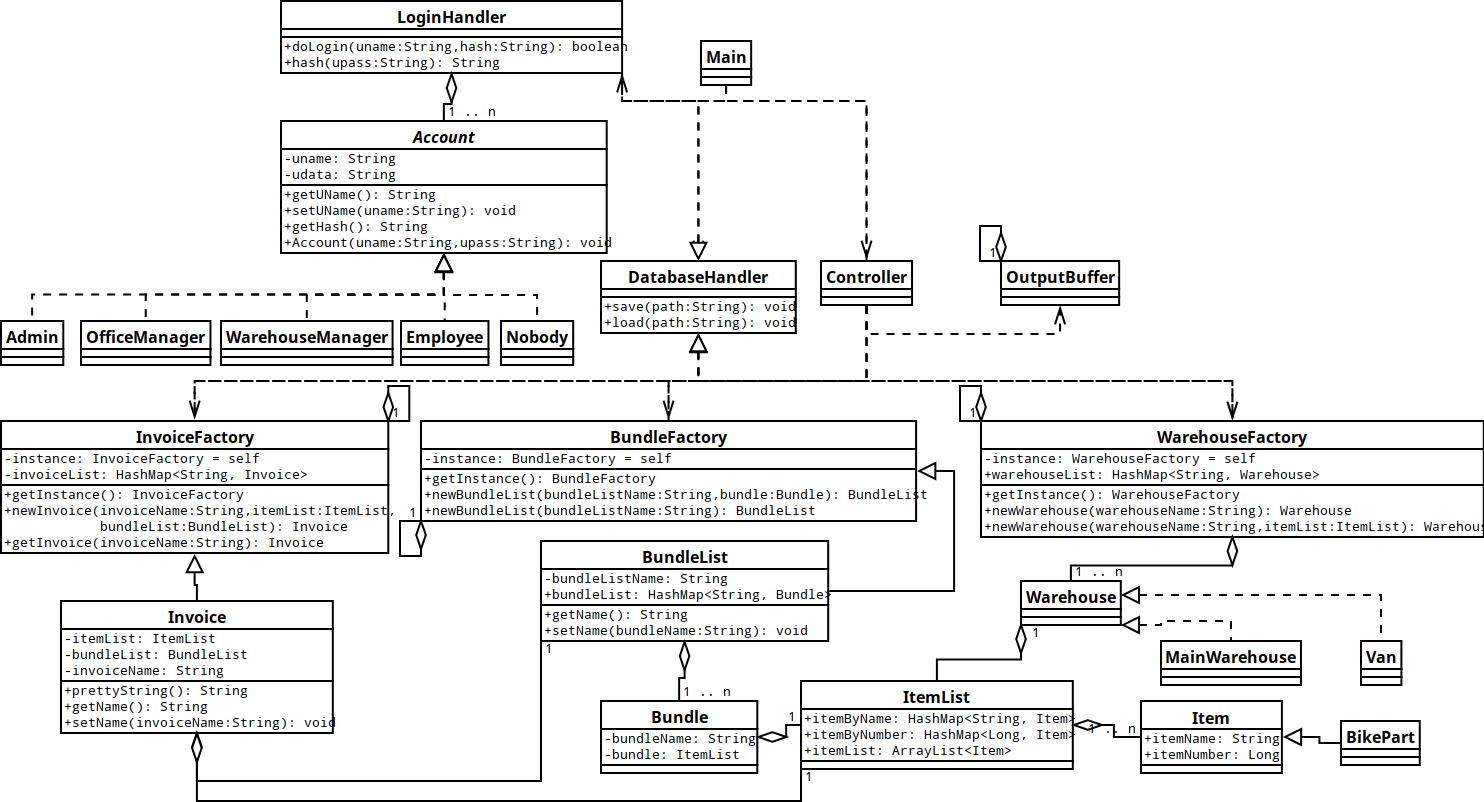
\includegraphics[width=\textwidth,height=\textheight,keepaspectratio]{../diagrams/image_versions/overview.png}
    \caption{Class hierarchy.}
\end{sidewaysfigure}

\clearpage

\subsection{Use Cases}

\begin{enumerate}
  \item \begin{description}
          \item [Case Name] System Administrator Login
          \item [Case Description] Ensure you are able to login properly to the System Administrator with Username: admin Password: minda and that the GUI switches to the correct panel.
        \end{description}
  \item \begin{description}
          \item [Case Name] Create Accounts
          \item [Case Description] Once logged into System Administrator create an account for each type of user(office manager, warehouse manager, sales associate, system administrator)  each user needs a username, password, phone number, and email.
        \end{description}
  \item \begin{description}
          \item [Case Name] Create Sales Associate Account
          \item [Case Description] During the create account process for a sales associate be sure to “link” each sales associate to a sales van.
        \end{description}
  \item \begin{description}
          \item [Case Name] Editing Accounts
          \item [Case Description] While logged into the System Administrator select to delete an existing account that was made, ensure that functionality works. Then on a different account reset the password to test that functionality.
        \end{description}
  \item \begin{description}
          \item [Case Name] Log In
          \item [Case Description] Ensure you are able to login properly to Office Manager, Warehouse Manager, and Sales Associate with the correct username and password. Ensure that the GUI switches to the correct panel based on what account you logged in as.
        \end{description}
  \item \begin{description}
          \item [Case Name] Examine Part Office Manager (Warehouse Manager has same capability)
          \item [Case Description] Once logged into Office Manager select to examine part; try each choice( part name, part number, or by “>,=,<”). Ensure that the correct parts are visible in the output after each choice.
        \end{description}
  \item \begin{description}
          \item [Case Name] Order Parts Office Manager
          \item [Case Description] Once logged into Office Manager set the minimum quantity for each part and ensure that once the supply is less than the minimum that a pop up notification becomes visible telling you to order the low quantity parts.
        \end{description}
  \item \begin{description}
          \item [Case Name] Query Inventory Office Manager
          \item [Case Description] Once logged into Office Manager and after being notified by the low quantity pop up. Select query inventory, and ensure a list of all parts that are less than and close(what classifies as close?) to their minimum quantities are shown in the output. Use this list to input what and quantity of each part you need to order.
        \end{description}
  \item \begin{description}
          \item [Case Name] Sales Commission Office Manager
          \item [Case Description] Once logged into Office Manager select sales commission, select a sales associate and start and end date to pull sales invoices from between those dates. Click on calculate and this will generate a paycheck for this employee between those dates which is 15\% of the total sales of that period for that associate.
        \end{description}
  \item \begin{description}
          \item [Case Name] Update Inventory Warehouse Manager
          \item [Case Description] Once logged into Warehouse Manager input the inventory file you want to read and ensure that the inventory for the main warehouse is updated; the new parts are added, existing parts attributes are updated, and that “ALL” warehouses with their corresponding parts price attributes are also updated. (Project 2)
        \end{description}
  \item \begin{description}
          \item [Case Name] Delivery Files Sales Associate
          \item [Case Description] Once logged into Sales Associate input the delivery file name you want to read and ensure that the correct parts are moved from and to the correct warehouses and the quantities (decremented/incremented) were updated correctly per warehouse.
        \end{description}
  \item \begin{description}
          \item [Case Name] Sales Invoice Sales Associate
          \item [Case Description] Once logged into Sales Associate select sales invoice and fill in the required information; shop to receive parts name, parts to be sold, and quantity sold of each part. Click create and ensure a sales invoice is created with the shop names and date sold at the top, followed by a list of the parts sold (part name, part number, sale price or list price, quantity) and at the bottom the total cost of all the parts. (These are used by Office Manager to calculate paychecks per sales associate).
        \end{description}
  \item \begin{description}
          \item [Case Name] GUI aesthetic check
          \item [Case Description] Check each tab within the GUI and ensure there is no typos or confusing placement of items within each tab.
        \end{description}
\end{enumerate}

\begin{figure}
  \centering
    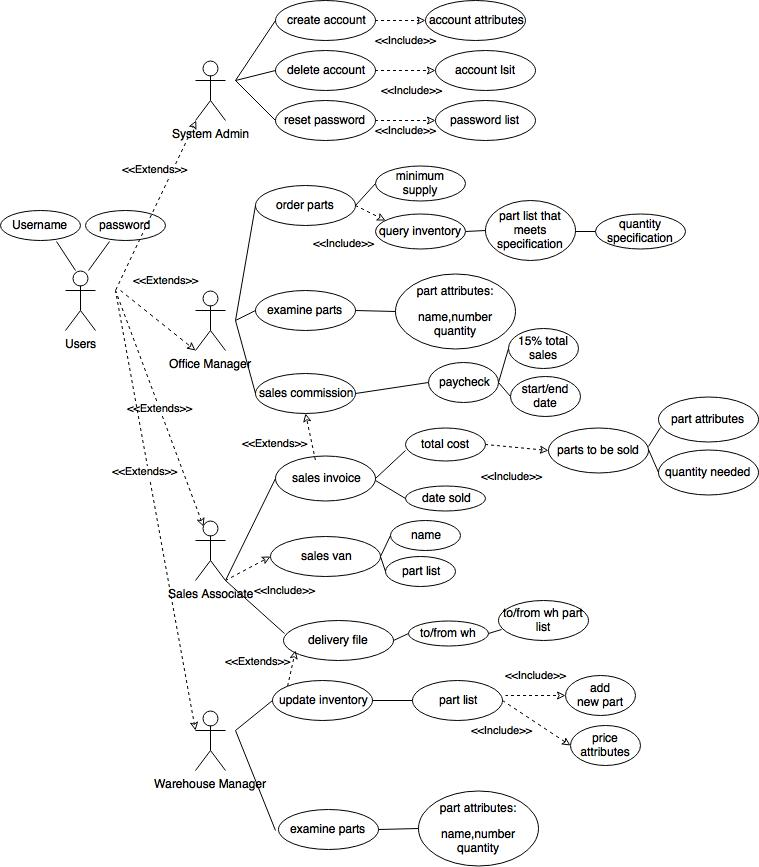
\includegraphics[width=\textwidth,height=\textheight,keepaspectratio]{../diagrams/image_versions/use_cases.jpg}
  \caption{General use case diagram.}
\end{figure}

%\begin{figure}[h]
%  \centering
%    \includegraphics[scale=0.5,keepaspectratio]{wmsequence.png}
%  \caption{Warehouse manager use cases.}
%\end{figure}

%\begin{figure}[h]
%  \centering
%    \includegraphics[scale=0.5,keepaspectratio]{ui.png}
%  \caption{The JavaFX UI for the project.}
%\end{figure}

\listoffigures

\listoftables

\end{document}
